\chapter{Foreword: Mechanics and Meta-information}

\section{Damage description}

Generally, I will call for you to describe your attacks hit.
However, in a fight it really only takes one or two solid hits with a weapon to kill someone.
To keep things at least half sensible with respect to how much damage a monster can soak, I'll use
  the following general guides when calling for the severity of blow your just dealt.

\begin{tabular}{|r|l|}
\hline
Remaining HP\dots & Described as \\
\hline
$0\%$    & Killing \\
$<25\%$  & Wounding \\
$<50\%$  & Connecting \\
$<75\%$  & Glancing \\
$<100\%$ & Absorbed \\
\hline
\end{tabular}

\newpage
\section{Speed Factor Initiative}

I'd like to use the Speed Factor Initiative rules with the Angry DM's modifier table.

For more, read:\newline\url{http://theangrygm.com/fine-i-wrote-about-speed-factor-initiative-in-dd-5e/}.

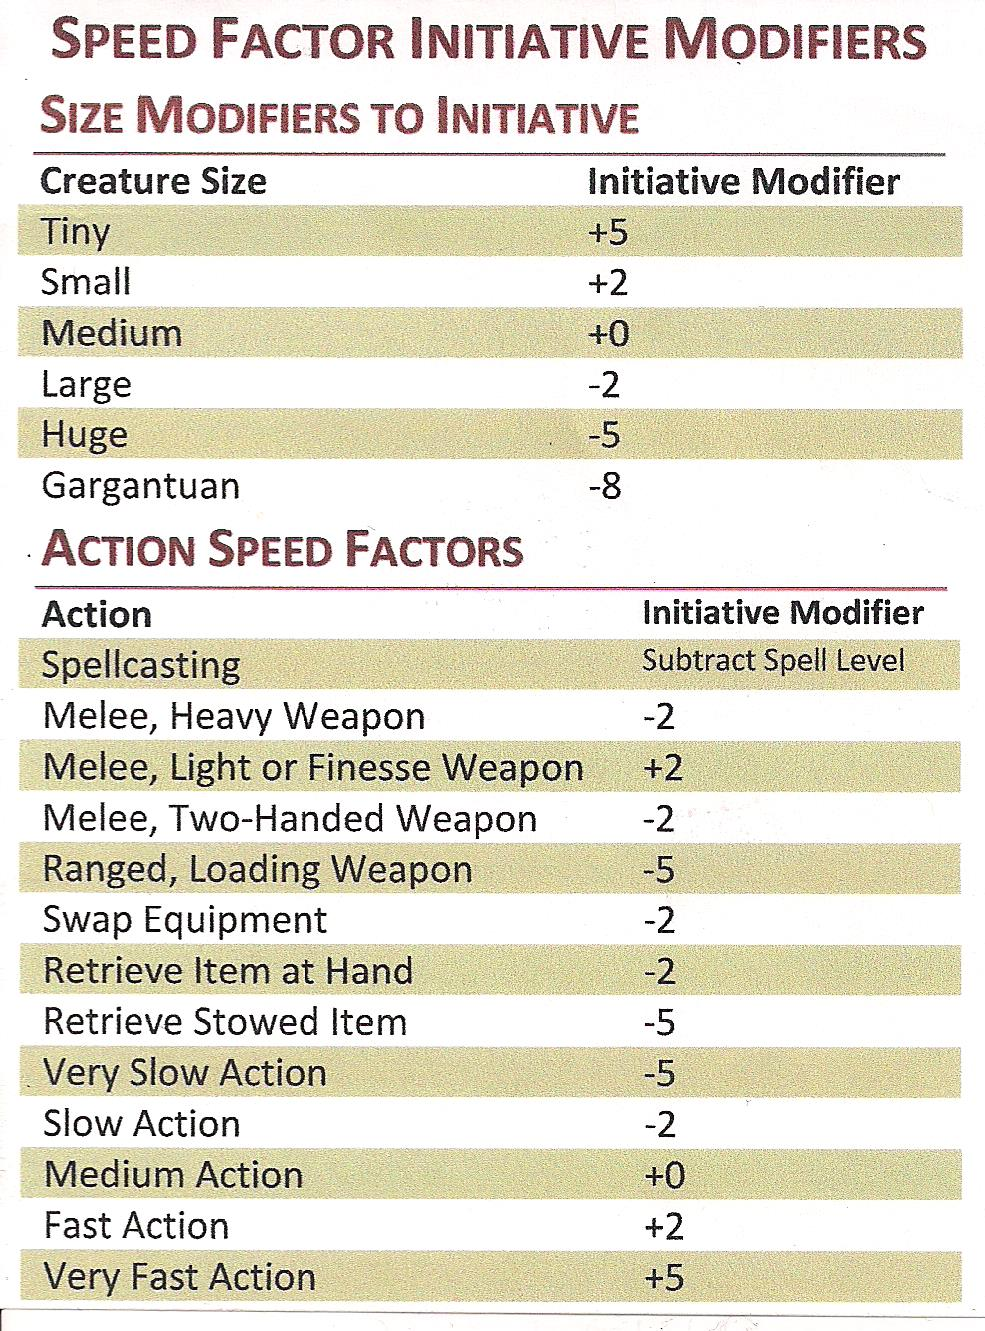
\includegraphics{img/speed-factor-initiative.jpeg}

\section{World map}
This is mostly as a note for me, but if it ever comes up on your next, a hex is 5 miles.
The PHB mentions that you can cover 18 / 24 / 30 miles a day at a slow / normal / fast pace,
  or 2 / 3 / 4 miles per hour.


\includegraphics[width=\linewidth,keepaspectratio=true]{img/maps/world-maps/Talaj.png}

\includegraphics[width=\linewidth,keepaspectratio=true]{img/maps/world-maps/Talaj2.png}

